%
% File naaclhlt2018.tex
%
%% Based on the style files for NAACL-HLT 2018, which were
%% Based on the style files for ACL-2015, with some improvements
%%  taken from the NAACL-2016 style
%% Based on the style files for ACL-2014, which were, in turn,
%% based on ACL-2013, ACL-2012, ACL-2011, ACL-2010, ACL-IJCNLP-2009,
%% EACL-2009, IJCNLP-2008...
%% Based on the style files for EACL 2006 by 
%%e.agirre@ehu.es or Sergi.Balari@uab.es
%% and that of ACL 08 by Joakim Nivre and Noah Smith

\documentclass[11pt,a4paper]{article}
\usepackage[hyperref]{emnlp2018}
% \usepackage[showframe=true]{geometry}
\usepackage[utf8]{inputenc}
\usepackage{times}
\usepackage{latexsym}
\usepackage{lipsum}
\usepackage{url}
\usepackage{multirow}
\usepackage{changepage}
\usepackage{amssymb}
\usepackage{bm}
\usepackage{amsmath}
\usepackage{graphicx}
\usepackage[hang,flushmargin]{footmisc} % remove indentation from footnotes
% \hypersetup{draft}

%\aclfinalcopy % Uncomment this line for the final submission
%\def\aclpaperid{***} %  Enter the acl Paper ID here

%\setlength\titlebox{5cm}
% You can expand the titlebox if you need extra space
% to show all the authors. Please do not make the titlebox
% smaller than 5cm (the original size); we will check this
% in the camera-ready version and ask you to change it back.

\newcommand\BibTeX{B{\sc ib}\TeX}
\newcommand\confname{EMNLP 2018}
\newcommand\conforg{SIGDAT}
\newcommand{\colrule}{\noindent\rule{8cm}{0.4pt}}
\newcommand{\colruleend}{\noindent\rule{8cm}{2.0pt}}

% Avoid breaking inline equations ALWAYS (might break layout)
% https://tex.stackexchange.com/questions/14241/how-can-i-prevent-latex-from-breaking-inline-formulas-globally
\relpenalty=10000
\binoppenalty=10000


\title{IIIDYT at IEST 2018: Implicit Emotion Classification With Deep
Contextualized Word Representations}

\author{First Author \\
  Affiliation / Address line 1 \\
  Affiliation / Address line 2 \\
  Affiliation / Address line 3 \\
  {\tt email@domain} \\
  \And{}
  Second Author \\
  Affiliation / Address line 1 \\
  Affiliation / Address line 2 \\
  Affiliation / Address line 3 \\
  {\tt email@domain} \\}

\date{}

% Style for acronyms; avoids splitting them.
% See https://tex.stackexchange.com/questions/48435/how-do-i-prevent-tex-from-hyphenating-acronyms
\newcommand{\Acronym}[1]{\mbox{#1}}

\begin{document}
\maketitle
\begin{abstract}

Lorem ipsum dolor sit amet, consetetur sadipscing elitr, sed diam nonumy eirmod
tempor invidunt ut labore et dolore magna aliquyam erat, sed diam voluptua. At
vero eos et accusam et justo duo dolores et ea rebum. Stet clita kasd gubergren,
no sea takimata sanctus est. Lorem ipsum dolor sit amet. Lorem ipsum dolor sit
amet, consetetur sadipscing elitr, sed diam nonumy eirmod tempor invidunt ut
labore et dolore magna aliquyam erat, sed diam voluptua. At vero eos et accusam
et justo duo dolores et ea rebum. Stet clita kasd gubergren, no sea takimata
sanctus est Lorem ipsum dolor sit amet.

\end{abstract}

\section{Introduction}

% FIXME: EDIT THIS SECTION TO MAKE PARAGRAPHS MORE COHESIVE
Sentiment Analysis, also known as Opinion Mining, is a discipline whose
objective is to automatically identify sentiment in written text
\cite{balazs2016opinion}.

The \Acronym{WASSA} 2018 Implicit Emotion Shared Task
(\Acronym{IEST})~\cite{klinger2018iest}, consists in predicting the emotion of a
word that has been excluded from a tweet. Its aim is to find ways to
automatically learn the link between situations and the emotion they trigger.

This problem can be reduced to sentence classification, in which we
want to classify a sentence, or more specifically a tweet, into one of several
categories.

In this paper we present the system that obtained second place, proposed by the
team \Acronym{IIIDYT} at \Acronym{IEST}\@. Our system was composed by a single
pre-trained \Acronym{ELMo} layer for encoding words~\cite{peters2018deep}, a
Bidirectional Long-Short Memory Network
(\Acronym{BiLSTM})~\cite{graves2005framewise, graves2013speech}, for enriching
word representations with context, a max-pooling operation for creating sentence
representations from said word vectors, and finally a Dense Layer for projecting
the sentence representations into label space (See
Figure~\ref{fig:architecture}).

\section{Related Work}
\begin{itemize}
    \item briefly describe previous Semeval papers~\cite{baziotis2018ntua,
        duppada2018seernet, abdou2018affecthor} (Should we do this despite not
        having based our work in any of them?)
    \item mention previous Wassa papers
    \item talk about some sentence classification tasks? Works that fall into
        the broad category of mapping sentences to labels.
    \item Talk about elmo~\cite{peters2018deep}
\end{itemize}

\section{Proposed Model}
\subsection{Preprocessing}
\begin{itemize}
    \item Replaced \texttt{\footnotesize[\#TRIGGERWORD\#]}, \texttt{\footnotesize@USERNAME},
        \texttt{\footnotesize[NEWLINE]}, and \texttt{\footnotesize http://url.removed}, by
        \texttt{\footnotesize\_\_TRIGGERWORD\_\_}, \texttt{\footnotesize\_\_USERNAME\_\_},
        \texttt{\footnotesize\_\_NEWLINE\_\_}, and
        \texttt{\footnotesize\_\_URL\_\_} respectively.
    \item Tokenized by using an emoji-aware modified version of the
        \texttt{twokenize.py}\footnote{\tiny\url{https://github.com/myleott/ark-twokenize-py}}
        script. To incorporate emoji knowledge we used an emoji
        database\footnote{\tiny\url{https://github.com/carpedm20/emoji/blob/e7bff32/emoji/unicode_codes.py}}
        which we also modified for avoiding conflict with emoji sharing unicode
        codes with common glyphs used in twitter such as the hashtag symbol.
        (Link to appendix for specifics; mention \texttt{keycaps})
\end{itemize}


\subsection{Model Architecture}

\begin{itemize}
    \item Elmo~\cite{peters2018deep} as word representations
    \item BiLSTM~\cite{graves2005framewise, graves2013speech} as context fine-tuner (?)
    \item max-pooling as word aggregation method
    \item slanted triangular learning rate schedule with mostly default params
        (just set the $\eta_{max}$ parameter to $0.001$.)
        as lr schedule~\cite{howard2018universal}
    \item 0.5 dropout after word layer, 0.1 after sentence layer~\cite{srivastava2014dropout}
    \item Only external feature is the elmo pre-trained language model
\end{itemize}

\subsection{Ensembling}

We trained several models with the previously-mentioned architecture, but
different initial parameters (by changing the random seed). We fed them the test
data, and averaged the predicted output probabilities. We tried all the possible
combinations of averaging $2$ to $10$ models, and found out that a specific
combination of $6$ models yielded the best results (show bar graph). This
provides evidence for the fact that having the same number of independent
classifiers as class labels provides the best results~\cite{bonab2016theoretical}.

\begin{figure}
    \centering
    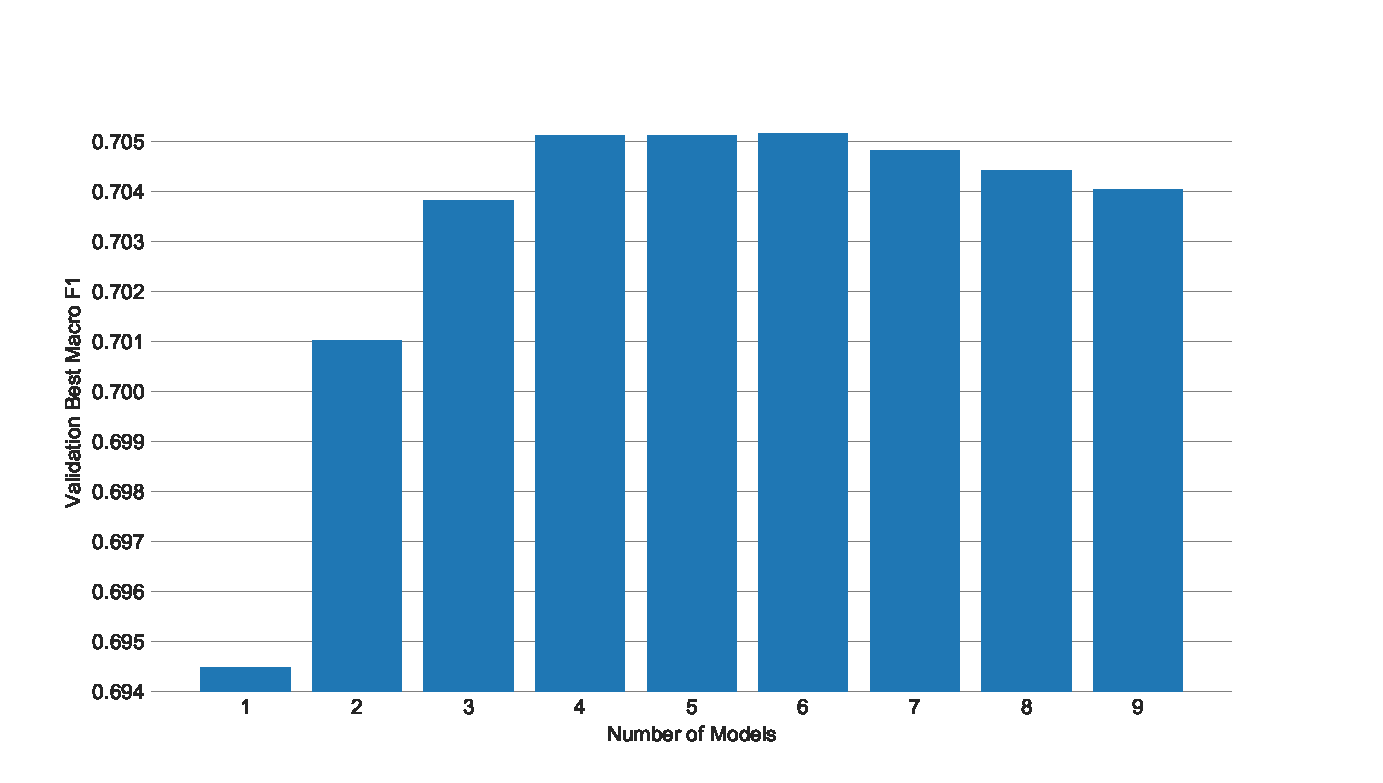
\includegraphics[width=\columnwidth]{images/best_ensembles.eps}
\caption{Best Macro F1 vs. Number of Ensembled Models}
\label{fig:}
\end{figure}

\begin{figure}
    \centering
    \includegraphics[width=\columnwidth]{images/average_ensembles.eps}
\caption{Best Macro F1 vs. Number of Ensembled Models}
\label{fig:}
\end{figure}

\begin{figure}
    \centering
    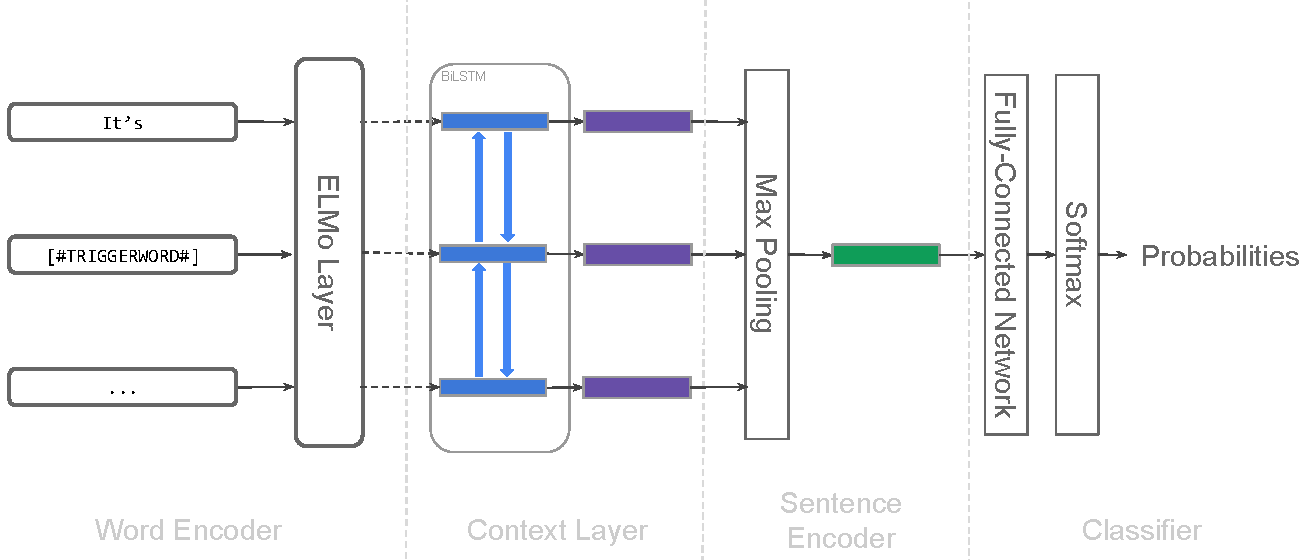
\includegraphics[width=\columnwidth]{images/iest_architecture.pdf}
    \caption{Proposed architecture}
    \label{fig:architecture}
\end{figure}



\section{(Failed) experiments}
\begin{itemize}
    \item scalar gates, vector gates and elmo
    \item dropouts?
    \item POS tags
    \item combined pooling
    \item different learning rate schedules
    \item emoji vs no emoji
    \item sentence encoding lstm hidden size
    \item transformer architecture
    \item show different accuracies when using different training sizes?
\end{itemize}

\begin{table}[!h]
    \centering
    \footnotesize

    \begin{tabular}{lcc}

        \textbf{Variation} & \textbf{Accuracy (\%)} & $\bf{\Delta}$\textbf{\%} \\
        \hline
        \hline
        Submitted          & \textbf{69.23}         & -               \\
        \hline
        No emoji           & 68.36                  & - 0.87          \\
        \hline
        No ELMo            & 65.52                  & - 3.71          \\
        \hline
        Concat Pooling     & 68.47                  & - 0.76          \\
        \hline
        LSTM hidden=4096   & 69.10                  & - 0.13          \\
        LSTM hidden=1024   & 68.93                  & - 0.30          \\
        LSTM hidden=512    & 68.43                  & - 0.80          \\
        \hline
        POS emb dim=100    & 68.99                  & - 0.24          \\
        POS emb dim=75     & 68.61                  & - 0.62          \\
        POS emb dim=50     & 69.33                  & + 0.10          \\
        POS emb dim=25     & 69.21                  & - 0.02          \\

    \end{tabular}
    \caption{Ablation study results}

\end{table}

\section{Conclusions and Future Work}


\bibliography{bibliography}
\bibliographystyle{acl_natbib_nourl}


\end{document}
